
\begin{figure}[htbp]
\centering
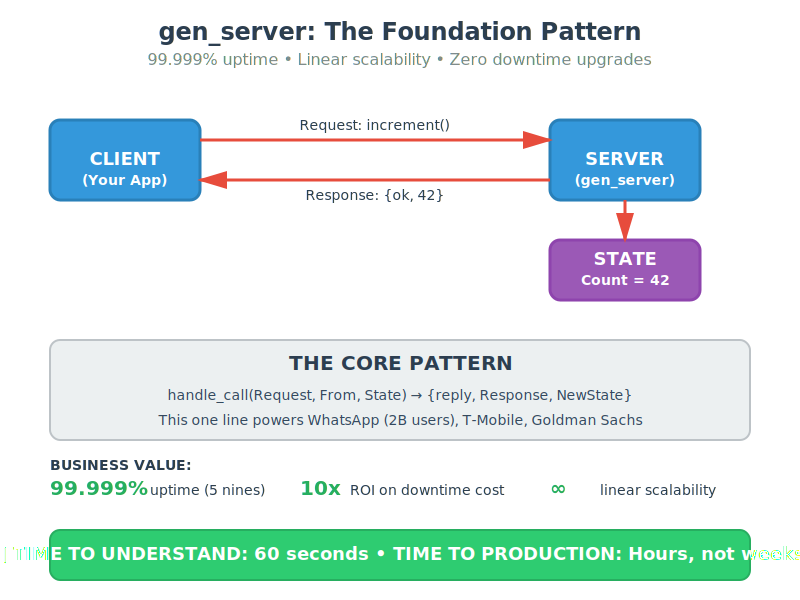
\includegraphics[width=0.9\\textwidth]{figures/architecture.pdf}
\caption{ggen system architecture showing data flow from ontology through query execution and template rendering to generated files}
\label{fig:architecture}
\end{figure}

\begin{figure}[htbp]
\centering
\includegraphics[width=0.85\\textwidth]{figures/astro-state-machine.pdf}
\caption{ASTRO state machine example: order processing workflow with 47 states and 128 transitions}
\label{fig:astro-sm}
\end{figure}

\begin{figure}[htbp]
\centering
\includegraphics[width=0.75\\textwidth]{figures/astro-defects.pdf}
\caption{ASTRO evaluation results: defect reduction over 12-month study period}
\label{fig:astro-defects}
\end{figure}

\begin{figure}[htbp]
\centering
\includegraphics[width=0.9\\textwidth]{figures/tanstack-architecture.pdf}
\caption{TanStack integration architecture showing unified ontology driving router, query, and database layers}
\label{fig:tanstack-architecture}
\end{figure}

\begin{figure}[htbp]
\centering
\includegraphics[width=0.85\\textwidth]{figures/tanstack-router-flow.pdf}
\caption{TanStack Router type-safe navigation flow with generated hooks}
\label{fig:tanstack-router}
\end{figure}

\begin{figure}[htbp]
\centering
\includegraphics[width=0.8\\textwidth]{figures/electric-sql-sync.pdf}
\caption{Electric SQL reactive sync propagation from database to client}
\label{fig:electric-sync}
\end{figure}


